% !TeX spellcheck = en_US
\chapter{Hadron Therapy}

\section{Introduction}
The National Cancer Institute define a tumor\cite{tumor} as “an abnormal mass of tissue that results when cells divide more than they should or do not die when they should”.
In a healthy body, cells grow, divide, and replace each other in the body. As new cells form, the old ones die. When a person has cancer, new cells form when the body does not need them. If there are too many new cells, a group of cells, or tumor, can develop.
A tumor develops when cells reproduce too quickly. Tumors can vary in size from a tiny nodule to a large mass, depending on the type, and they can appear almost anywhere on the body.
There are three main types of tumor:
\begin{itemize}
\item \textbf{Benign}: These are not cancerous. They either cannot spread or grow, or they do so very slowly. If a doctor removes them, they do not generally return.
\item \textbf{Premalignant}: In these tumors, the cells are not yet cancerous, but they have the potential to become malignant.
\item \textbf{Malignant}: Malignant tumors are cancerous. The cells can grow and spread to other parts of the body.
\end{itemize}
Radiation therapy is the medical use of ionizing radiation to treat cancer. In conventional radiation therapy, beams of X rays (high energy photons) are produced by accelerated electrons and then delivered to the patient to destroy tumour cells. Using crossing beams from many angles, radiation oncologists irradiate the tumour target while trying to spare the surrounding normal tissues. Inevitably some radiation dose is always deposited in the healthy tissues.
When the irradiating beams are made of charged particles (protons and other ions, such as carbon), radiation therapy is called hadron therapy\cite{radiationtherapy}. The strength of hadron therapy lies in the unique physical and radiobiological properties of these particles; they can penetrate the tissues with little diffusion and deposit the maximum energy just before stopping. This allows a precise definition of the specific region to be irradiated. The peaked shape of the hadron energy deposition is called Bragg peak and has become the symbol of hadron therapy. With the use of hadrons the tumour can be irradiated while the damage to healthy tissues is less than with X-rays.

\section{Interaction between matter and charged particles}
Charged particles with mass greater than the one of the electron lose energy in matter through ionization.
A classic calculation for the energy lost in ionization can be done taking into account two assumptions:
\begin{itemize}
	\item the speed of the atomic electron is negligible compared to the one of the incident particle;
	\item the mass of the incident particle is big in relation to the target mass. This means that the incident particle for each single hit receives a small amount of momentum and thus the direction of flight does not changes.  
\end{itemize}
\noindent This hypothesis is valid keeping into consideration that the mass of the electron is 0.51 MeV, a muon has mass 105.6 MeV, for a proton it is 938.2 MeV and for a carbon ion ${}^{12}$C it is 11177.9 MeV.
\newline
The classic calculation results in the Bethe-Block formula in equation \ref{eq:bethe} that describes the average energy loss in the target for unit of length, also called stopping power.
\begin{equation}\label{eq:bethe}
	-\dfrac{\mathrm dE}{\mathrm dx} = 2 \pi N_{a} r_{e}^{2} m_{e} c^{2} \rho \dfrac{Z}{A}  \dfrac{z^{2}}{\beta^{2}}\left[\ln\left(\dfrac{2m_{e} \gamma ^{2} v^{2} W_{max}}{W^{2}}\right) - 2\beta^{2} - \delta 2\frac{C}{Z}\right]
\end{equation}
\noindent In equation \ref{eq:bethe}:
\begin{itemize}
	\item $N_a$: is the Avogadro number;
	\item $r_e$: is the classical radius of the electron;
	\item $m_e$: is the mass of the electron;
	\item $\rho$: target density;
	\item $Z $: target atomic number;
	\item $A $: target atomic mass;
	\item $W $: target average ionization energy;
	\item $z $: incident particle charge;
	\item $W_{max} $: maximum energy transferred in a collision; 
	\item $\delta $: polarization parameter in target
	\item $c/z $: core electrons shielding parameter 
	\item $\beta = v/c $
\end{itemize}
\noindent The stopping power depends by the target mass, atomic number, density and average ionization energy (A, Z, $\rho$, W). To overcome and eliminate this dependence it was defined the massic stopping power in equation \ref{eq:stoppingpower} that is measured in MeV/(g cm${}^2$)
\begin{equation}\label{eq:stoppingpower}
	\delta = - \frac{1}{\rho} \frac{dE}{dx}
\end{equation}
\noindent In figure it can be seen the trend of the massic stopping power of a $\mu^+$ passing through a copper layer.
\begin{figure}[H]
	\centering
	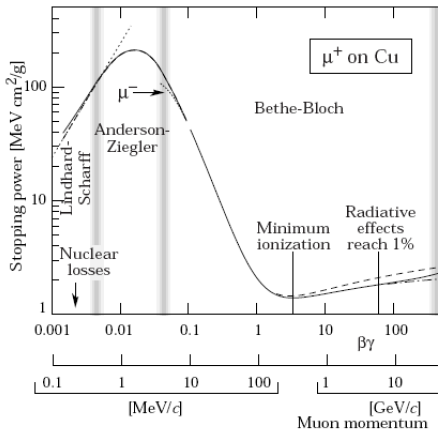
\includegraphics[width=0.7\linewidth]{IMG/ch1/MassicStoppingPower}
	\caption{Massic Stopping power in function of the $\mu^+$ momentum passing through a copper layer}
	\label{fig:massicstoppingpower}
\end{figure}
\noindent In the trend of the stopping power in function of the momentum can be noted a de-growth for low momentum values that is due to the term $\frac{1}{\beta^2}$ in equation \ref{eq:bethe}; the stopping power decreases until it reaches a minimum, and then slowly grows back.
\newline
The average path (range) of a charged particle can be calculated by integrating the stopping power along the "walk".
\begin{equation}\label{eq:range}
	R=\int_{E_i}^{0} \frac{1}{\frac{dE}{dx}}dx
\end{equation}
\noindent The range depends approximately on the A / Z ratio of the material and grows approximately with the square of the initial kinetic energy of the charged particle. The accrual
of energy loss increases as the kinetic energy of the particle decreases with the depth of penetration, with a rapid ascent at the end of the path. The density of ionization of the charged particles along their path in the medium is therefore
characterized by a plateau followed by a pronounced maximum towards the end of range, called Bragg peak, which is located at an energy-dependent depth initial kinetics of the incident particle, as shown in figure \ref{fig:braggpeak}.
If more particles are considered then it should be kept in mind
the statistical fluctuations on the collisions of the particles and on the energy transferred for each collision: these fluctuations are well described by the Landau distribution \cite{landau}
, generate uncertainty about the distance reached by the particles ("straggling"). Beyond all these considerations we must not neglect the possible interactions with the nuclear components of the matter crossed. One effect is enlargement
lateral of the beam due to the interaction with the Coulomb fields of the nuclei that it is inversely proportional to the mass of the incident particle. The second effect it is due to the fragmentation of the primary bundle and/or of the nuclei of the material passed through due to nuclear interactions. The fragmentation cross section becomes relevant for ions heavier than the proton, such as carbon ions or heavier, and causes a decrease in the number of particles incident along the path
and the development of secondary fragments. The fragments produced deposit theirs energy deeper than the Bragg peak giving rise to a queue in the distribution.
\begin{figure}[H]
	\centering
	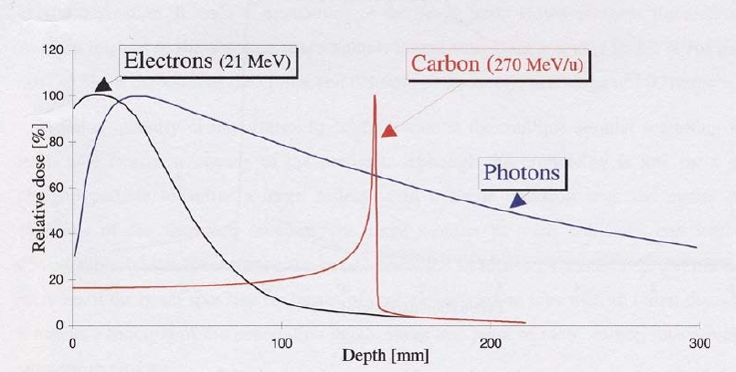
\includegraphics[width=0.7\linewidth]{IMG/ch1/BraggPeak}
	\caption{Dose profile for a 21MeV electron, 270MeV/u carbon ion and photon beam}
	\label{fig:braggpeak}
\end{figure}  

%\begin{equation}\label{eq:bethe2}
%	W_{max} = \dfrac{2m_{e} c^{2} \eta^{2}}{1+2s \sqrt{1+\eta^{2}} + s^{2}};\qquad s=m_{e}/M;\eta=\beta\gamma.
%\end{equation}


\section{Effects of radiations on biological systems}
Radiation is energy. A charged particle when it interacts with the human body loses its energy. The measurement and calculation of the ionizing radiation dose absorbed by an object is called radiation dosimetry.
\newline
Thus the dose (D) can be defined as the energy absorbed divided by the object mass.
\begin{equation}\label{eq:dose}
	D\left[Gy \right] =\frac{dE}{dm}
\end{equation}
In the I.S. the unit of measure is the Gray(Gy)[JKg${}^{-1}$]=1J/1Kg.
\newline
It is also common the use of an equivalent dose (H=DxW$_1$) where W$_1$ is a weight that depends on the type of particle (photon, electron, neutron, proton, heavy charged particle, ecc...). The unit of measure of the equivalent dose is the Sievert(Sv)[JKg${}^{-1}$], although in the past it was used the rem[1Sv=100rem].
\newline
When monitoring the dose absorbed by an human body it must me considered that not every organ has the same resistance to radiation, thus it is used the effective dose (E=HxW$_2$) which is the equivalent dose multiplied by the weight W$_2$ which depends on the part of the body interested by the radiations.
\newline
\noindent The energy deposition is strictly dependent by the type of radiation like photons, electrons or heavy charged particles. As shown in figure \ref{fig:braggpeak} the relative dose percentage delivered by the photons is maximum at low depth and then has an exponential decrease as the thickness of the tissue increases.
The dose profile in function of the depth for heavy charged particles (as carbon ions) is characterized by a low dose at the beginning of the tissue and then by a extremely peaked spike at the end of their travel (Bragg peak).
Since the depth of this peak depends by the beam energy, this can be tuned to deliver the dose at different depths.
Moreover, thanks to the high mass of the particles, it is possible to greatly reduce the lateral diffusion effects thus saving the healthy tissues and the critical structures near the target.
\begin{figure}[H]
	\centering
	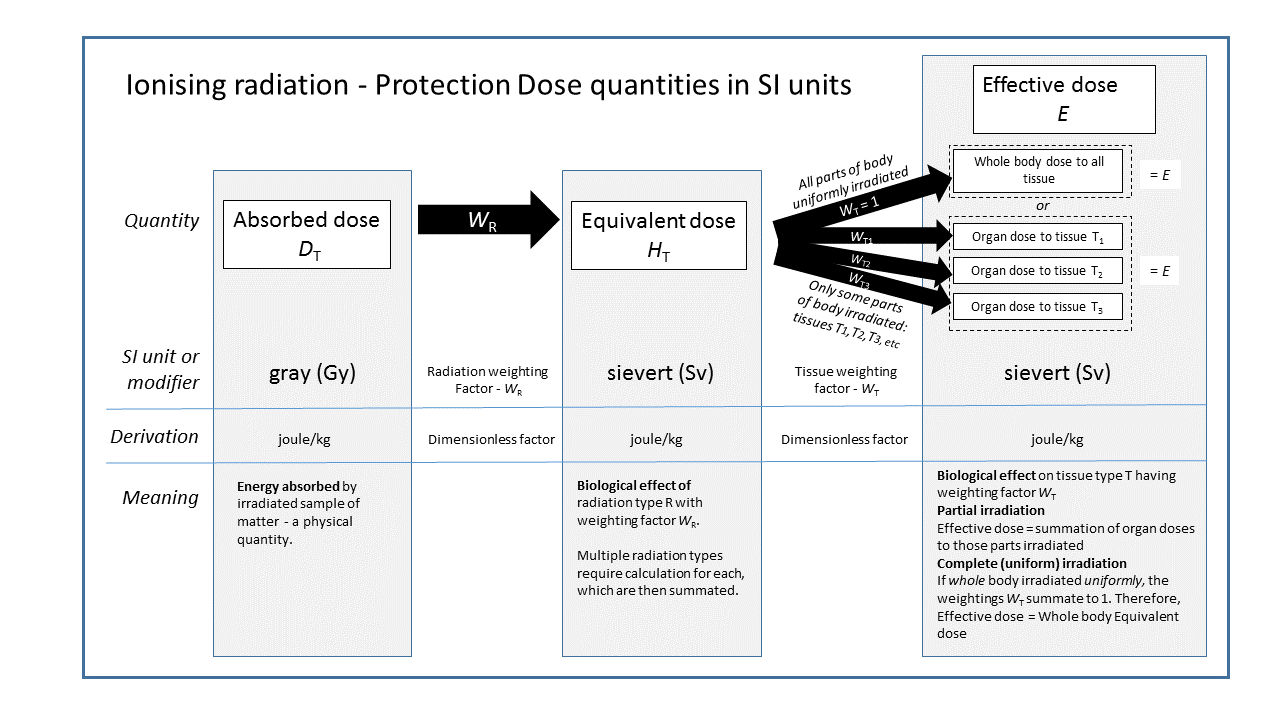
\includegraphics[width=0.7\linewidth]{IMG/ch1/SIRadiationDoseUnits}
	\caption{Absorbed, equivalent and effective dose units and meanings}
	\label{fig:SIRadiationDoseUnits}
\end{figure} 
\noindent With heavy charged particles is therefore possible to accurately focus the beam for a selected depth; this is not possible with other sources of radiation.
\newline
The different rates of energy loss at different depths for photons and heavy charged particles produce different dose distributions as shown in figure \ref{fig:Dose}.
\begin{figure}[H]
	\centering
	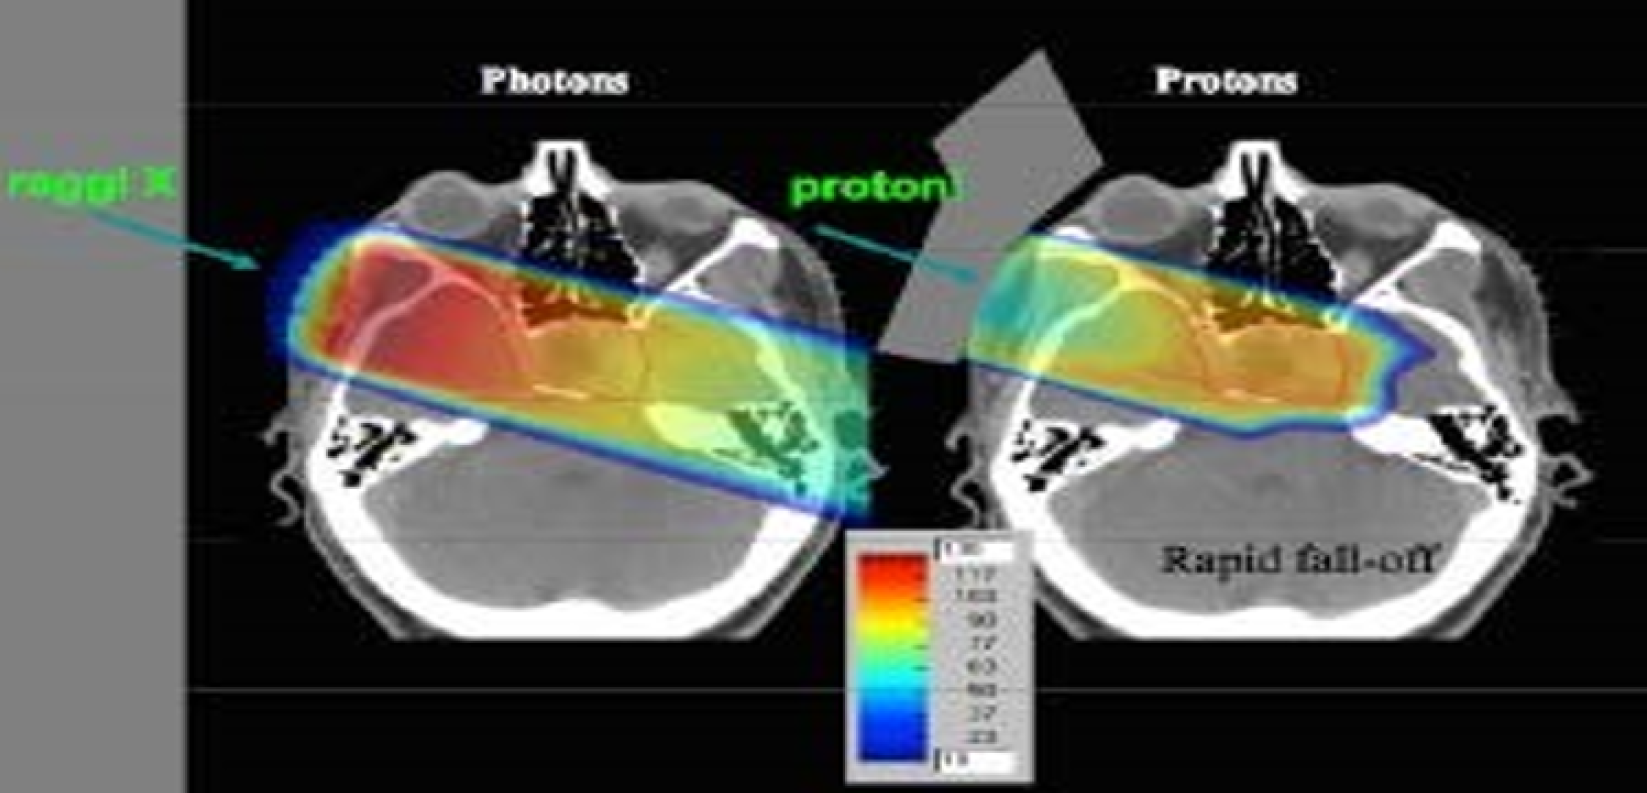
\includegraphics[width=0.7\linewidth]{IMG/ch1/Dose}
	\caption{Example of a dose distribution for a photon beam on the left and for a proton beam on the right}
	\label{fig:Dose}
\end{figure}

\noindent The energy released by the charged particles can cause both direct and indirect effects.
The direct ones are the interactions between the radiation and the biological molecules; this generates breaking points in the nucleotide chain of the DNA.
The indirect effects are the interactions, with production of free radicals, between radiations and water molecules inside the cell.
After that the free radicals interact with the biological molecules producing chemical alterations that can generate the inactivation of the cell cycle.
Damage to DNA molecules is considered the most important since it can lead to the cell's inability to reproduce and cell death\cite{cells}.
\newline
Irradiation can produce various types of alterations in the DNA structure:
\begin{itemize}
	\item \textbf{Single Strand Break} (SSB) when the nucleotide is damaged on a single DNA filament.
	\item \textbf{Double Strand Break} (DSB) when two or more nucleotide are damaged on both DNA filaments. 
\end{itemize}
Following the damage, there are several scenarios:
\begin{itemize}
	\item \textbf{Complete repair}, a situation that occurs for the majority of minor alterations (SSB), after which the cell resumes its normal activity.
	\item \textbf{Wrong repair}, in which the cell repairs its damage but not comprehensively. This can lead to the impossibility of replication of the cell or to its death by apoptosis. In some cases the cell may be able to divide, but by passing on a genetic mutation.
	\item \textbf{Unrepairable damage}, in this scenario the cell dies within a few hours due to the release of lytic enzymes or dies on the occasion of the first mitotic division. This situation occurs mainly in the case of DSB.
\end{itemize}
The cellular response to radiation depends in a complex way on the absorbed dose. In radiobiology, the biological efficacy of a radiation dose is studied by measuring cell survival as a function of the dose irradiated on the sample. The main physical factor on which biological damage depends, for the same dose administered, is the "Linear Energy Transfer" (LET)\cite{let}:   
\begin{equation}\label{eq:let}
	LET=\frac{dE}{dx}
\end{equation}
\noindent The LTE is defined as the average ionization density along the trail of a particle and is measured in keV/$\mu m$.
Radiations with high LET have, considering fixed the absorbed dose, a greater biological effect compared to the ones with low LET.
This happens because a higher ionization density imply a greater probability of unrepairable damages, like DSB.
The biological effect of a radiation is quantified in terms of Relative Biological Efficiency (RBE), defined as the ratio between the dose required to obtain a specific effect respectively with a reference radiation and with the radiation in question.
\begin{equation}\label{eq:rbe}
	RBE=\frac{D_{ref}}{D_{test}}
\end{equation}
\noindent The reference radiation $D_{ref}$ is commonly represented by a 250 keV X-ray beam, while $D_{test}$ corresponds to the dose of the radiation under examination.
\begin{figure}[H]
	\centering
	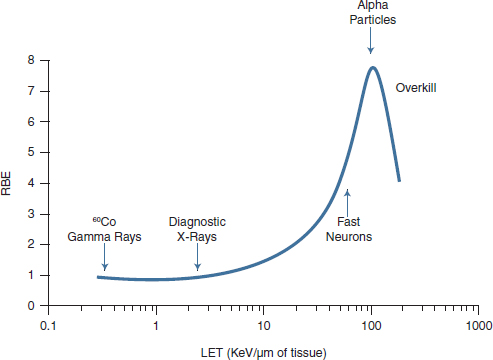
\includegraphics[width=0.7\linewidth]{IMG/ch1/RBE}
	\caption{RBE in function of the LET}
	\label{fig:rbe}
\end{figure}
\noindent In figure \ref{fig:rbe} it can be seen how the RBE changes i function of the radiation LET. From the graph it can be noted that the RBE growth, in function of the LET, starts for values near 1 keV/$\mu m$ and reaches a maximum near 100 keV/$\mu m$. For even higher LET values the RBE decreases, this is caused by a biological saturation effect that happens for high dose (overkill). 
10 MeV carbon ions have a LET of 170 keV/$\mu m$, this correspond to a RBE of 7. This is one of the reasons why therapies based on the use of carbon ions have been developed, which at the same dose, produce greater biological effects and are more effective in the treatment of radio-resistant tumors.


\section{Dose distribution systems in hadron therapy}
The physical and biological advantages of therapies with charged particles described in the previous paragraphs allow to obtain a precise conformation of the dose to the tumor, while minimizing the risk of side effects due to the irradiation of surrounding healthy organs.
These advantages are nowadays exploited in the treatment of delicate tumors in the proximity of organs at risk, pediatric tumors where the risk of side effects must be minimal, and radio-resistant tumors.
The number of patients treated with protons or carbon ions is growing each year as it can be seen in figure \ref{fig:patientstreated}
\begin{figure}[H]
	\centering
	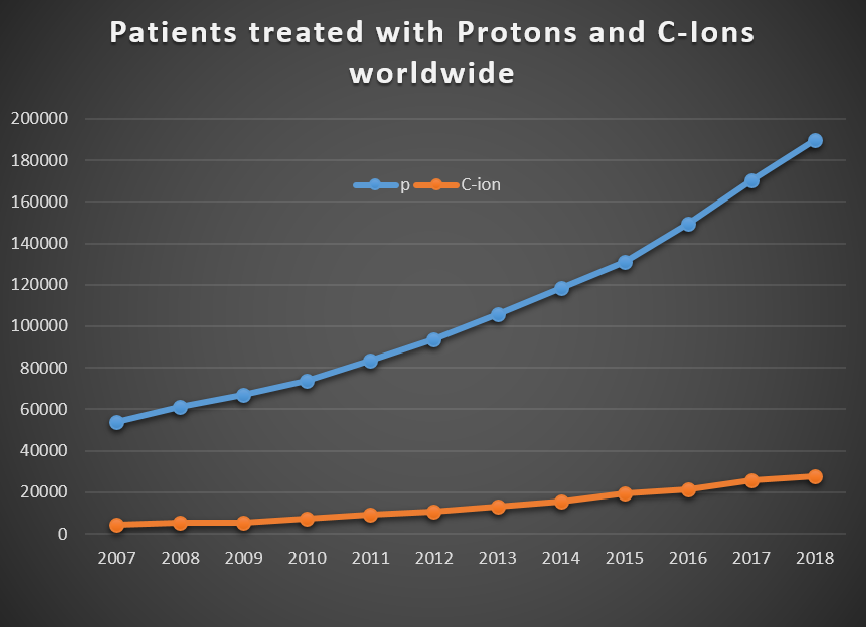
\includegraphics[width=0.7\linewidth]{IMG/ch1/PatientsTreated}
	\caption{Number of patients treated with annually with protons and carbon ions}
	\label{fig:patientstreated}
\end{figure}
This numbers, even if are growing, are still a small fraction of the total number of tumors treated with external radiation; X-ray being the main

\subsection{Passive dose distribution systems}

\begin{figure}[H]
	\centering
	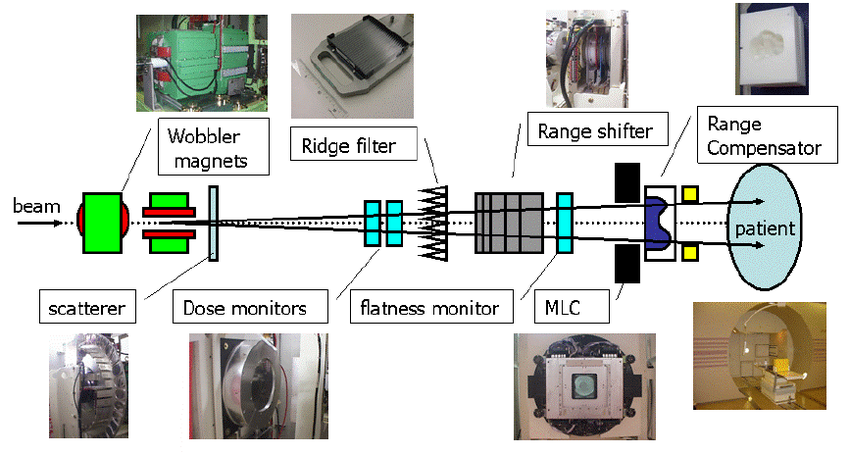
\includegraphics[width=0.7\linewidth]{IMG/ch1/Basic-design-of-irradiation-system-for-hadron-therapy}
	\caption{Basic design of passive dose distribution system for hadron therapy used to adapt the dose to the form of the tumor}
	\label{fig:passive}
\end{figure}
\subsection{Active dose distribution systems}

\subsection{Treatment Planning System}

\section{Beam monitoring}

\subsection{Silicon detectors}
















































